\documentclass[11pt,a4paper]{article}
\usepackage[T1]{fontenc}
\usepackage[utf8]{inputenc}
\usepackage{lmodern,microtype}
\usepackage[a4paper,margin=27mm,headheight=15pt]{geometry}
\usepackage{amsmath,amssymb,amsthm,mathtools,bm}
\usepackage{booktabs,array,longtable,graphicx,xcolor}
\usepackage{enumitem,fancyhdr}
\usepackage[hyphens]{url}
\usepackage[colorlinks=true,linkcolor=blue!45!black,citecolor=blue!45!black,urlcolor=blue!55!black]{hyperref}
\usepackage[nameinlink,noabbrev]{cleveref}
\definecolor{ink}{HTML}{133247}
\definecolor{accent}{HTML}{007F86}
\newtheorem{theorem}{Theorem}[section]
\newtheorem{lemma}[theorem]{Lemma}
\newtheorem{proposition}[theorem]{Proposition}
\newtheorem{corollary}[theorem]{Corollary}
\theoremstyle{definition}
\newtheorem{definition}[theorem]{Definition}
\newtheorem{example}[theorem]{Example}
\theoremstyle{remark}
\newtheorem{remark}[theorem]{Remark}
\DeclareMathOperator{\rank}{rank}
\DeclareMathOperator{\rad}{rad}
\DeclareMathOperator{\im}{im}
\DeclareMathOperator{\Sp}{Sp}
\DeclareMathOperator{\GL}{GL}
\DeclareMathOperator{\Mat}{Mat}
\DeclareMathOperator{\TV}{TV}
\newcommand{\F}{\mathbb F}
\newcommand{\E}{\mathcal E}
\newcommand{\gb}[2]{\genfrac{[}{]}{0pt}{}{#1}{#2}_q}
\setlength{\emergencystretch}{2em}
\setlength{\parskip}{3pt}
\setcounter{tocdepth}{1}
\setlist{itemsep=2pt,topsep=4pt}
\pagestyle{fancy}
\fancyhf{}
\fancyhead[L]{\small\color{ink}Exact symplectic compression laws}
\fancyhead[R]{\small Research note}
\fancyfoot[C]{\thepage}
\hypersetup{pdftitle={Exact symplectic compression laws},pdfauthor={Research prepared for Vladimir Reshetnikov},pdfsubject={Arbitrary frames, minimal realization dimension, and sharp finite-field asymptotics}}

\begin{document}
\begin{center}
{\small\sffamily\color{accent}FINITE GEOMETRY \quad / \quad RANDOM MATRICES \quad / \quad GRH METHOD TRANSFER}\par
\vspace{9mm}
{\LARGE\bfseries\color{ink}Exact symplectic compression laws}\par
\vspace{3mm}
{\large Arbitrary frames, minimal dimension, and sharp asymptotics}\par
\vspace{7mm}
Research prepared for Vladimir Reshetnikov\par
26 November 2026
\end{center}
\vspace{4mm}

\begin{abstract}
We determine the complete distribution of $Y^{\mathsf T}JgX_0$ when $g$ is uniform in a finite symplectic group and the two fixed injective frames have arbitrary prescribed alternating Gram matrices. The answer depends on three easily computed integers: half the rank of the combined Gram matrix and the dimensions of its radical inside the two coordinate blocks. An explicit positive sum counts possible relation spaces; multiplying by the classical prescribed-frame count gives the joint law of the observed matrix and the intersection dimension of the two frames. In particular, prescribed internal and cross pairings have an injective two-frame realization in smallest possible ambient dimension $2(s+\max(t_0,t_1))$.

For fixed frame dimensions and fixed field, we compute the first correction to independent uniform entries. The full total variation distance is asymptotic to an explicit positive constant times $q^{-2n}$, where the ambient dimension is $2n$. An exact two-plane example shows that equal-rank matrices can have different likelihoods and identifies the optimal distinguishing event. All results include characteristic two.

The finite-field compression method inside \texttt{grh-lean} motivates this work. The result extends the supplied ProveIt calculations from isotropic or Lagrangian output to two arbitrary restricted forms. Its proof is unconditional and uses classical finite symplectic geometry. The exact extension and its consequences are new relative to the inspected collection; worldwide publication priority is not established. Independent exhaustive enumeration and an executable minimum-dimension construction accompany the proof.
\end{abstract}

\vspace{2mm}
\noindent\textbf{Main results.} The complete joint law is Theorem~\ref{thm:complete-law}; the minimum-dimension formula is Theorem~\ref{thm:minimum-dimension}; sharp fixed-size asymptotics and an exactly solved example follow in Section~\ref{sec:asymptotics}.
\tableofcontents
\newpage

\section{From the supplied proof to a finite geometric problem}
\label{sec:context}

\subsection{What was inspected}

The source is \texttt{lsernau/grh-lean} at commit
\texttt{72fead102f663d5c7a407964a13dc0cf9d977207}. Its public statements assert the Riemann hypothesis and GRH for Dirichlet $L$-functions, including imprimitive characters. The exported statements do not assert arbitrary Artin or automorphic GRH. The repository describes a Lean~4 development with axiom dependencies \texttt{propext}, \texttt{Classical.choice}, and \texttt{Quot.sound}; its reported compiler and independent-kernel checks were not rerun for this note \cite{grh}.

The supplied Wikipedia page describes the November 2026 announcement and the relationship between critical-line zeros and prime-counting errors \cite{wiki}. It provides orientation; the exact scope and transferable mechanism used here come from the source files. The new theorem below uses no analytic statement about $L$-functions.

The ProveIt comparison is pinned to commit \texttt{041d80325417}
(the full identifier appears in the references). Its index contains 61 organized packets and a merged article. Its nested incoming directory contains 48 additional archives. The latter were read from cached bytes whose Git blob hashes were checked against the current repository. The merged article explicitly describes itself as a consolidation rather than an independent verification \cite{proveit}.

\subsection{The source mechanism}

The reading guide organizes the analytic proof around three inputs: short integral forms, enough independent forms obtained through a second moment, and a lower bound for a twisted Gram determinant. A common main term cancels in the upper and lower estimates. The resulting one-sided prime remainder bound is converted into zero exclusion through a Landau argument and a choice of quadratic twist. The files \texttt{New/Reduction/MainInequality.lean} and \texttt{New/Reduction/Zeros/Criterion.lean} expose those two final interfaces \cite{grh}.

The present transfer begins earlier, in
\texttt{New/Spanning/SecondMoment/PositiveType.lean}. In mathematical notation, its finite-field statement is as follows. Let $G$ be a finite group, $\pi:G\to\GL_N(\F_q)$ a representation, and $A_0,A_1$ two $N\times m$ matrices. Let $\Theta:G\to\mathbb R_{\ge0}$ be of positive type, so that
\[
 \Theta(a^{-1}b)=\langle u_a,u_b\rangle
\]
for a family of vectors in a complex Hilbert space. If each nonzero source vector has weighted stabilizer mass at most $Y$, both under $\pi$ on the first frame and under its contragredient on the second, then
\begin{equation}\label{eq:source-bound}
 q\sum_{\det(A_1^{\mathsf T}\pi(g)A_0)=0}\Theta(g)
 \le 2\sum_g\Theta(g)+q^{m+N/2}Y.
\end{equation}
The proof realizes a bilinear additive-character sum as an inner product of orbit sums. Their squared norms are stabilizer masses. Cauchy--Schwarz and finite Fourier orthogonality then count kernel vectors.

This gives a concrete question independent of RH: when a group acts on a finite vector space, what does a small matrix of pairings reveal about that action? The source controls singularity. ProveIt already develops full-law Fourier estimates and higher kernel moments. Here we calculate the entire law for uniform symplectic actions by counting its fibers exactly.

\subsection{The precise increment over ProveIt}

The merged article's symplectic section gives a generic estimate and an exact isotropic boundary law. In our ambient-dimension notation, its generic bound is
\[
 d_{\mathrm{TV}}\bigl(\mathcal L(Y^{\mathsf T}JgX_0),U_{a,b}\bigr)
 \le Cq^{-(2n+1-a-b)/2},\qquad a+b\le2n,
\]
where $U_{a,b}$ is the uniform distribution on all $a\times b$ matrices. Its Question \texttt{spn:q:symplectic} asks for the effects of general restricted alternating forms \cite{proveit}.

The later packet \emph{Symplectic rank blindness} computes exact matrix likelihoods for a Lagrangian projection and arbitrary input form. It also shows that rank statistics can become asymptotically unable to distinguish distributions whose full matrix laws remain separated. Its stated remaining case has both compressed spaces arbitrary \cite{rankblind}.

Theorem~\ref{thm:complete-law} allows arbitrary forms on \emph{both} frames and arbitrary rectangular sizes. It additionally retains the dimension of their intersection. Theorem~\ref{thm:minimum-dimension} extracts the exact realizability obstruction, and Section~\ref{sec:asymptotics} determines the sharp correction to uniformity for fixed frame sizes. This settles the missing exact finite-dimensional extension; it does not classify every regime in which the two sizes grow with the ambient dimension.

\subsection{Classical ingredients and novelty boundary}

The proof rests on standard symplectic basis extension, prescribed-Gram frame counts, and Gaussian binomial coefficients. In particular, classifying a tuple by its kernel and induced form is classical: Guralnick, Larsen, and Tiep use precisely this orbit mechanism in Lemma~2.6 \cite{glt}. The new calculation here imposes separate injectivity on two blocks, evaluates the resulting transverse-kernel coefficient, and turns it into a joint probability law and a sharp realization formula.

Related finite-geometry work counts pairs of subspaces with specified disjointness and nondegeneracy properties \cite{deboeck}; form-prescribed uniform sampling is studied in \cite{ishizuka}; symplectic refinements of rectangular-matrix association schemes appear in \cite{zhang}. Those comparisons keep the novelty claim specific. The combined theorem was not located in the targeted search and is absent from the inspected ProveIt predecessors. No claim is made that the underlying orbit classification or symplectic geometry is new.

\section{The complete law of an arbitrary symplectic compression}
\label{sec:complete-law}

Let $q$ be a prime power. All spaces and matrices in this section are over
$\mathbb F_q$. An alternating form means a bilinear form $B$ satisfying
$B(x,x)=0$ for every $x$. Its matrix therefore has zero diagonal as well as
$H^{\mathsf T}=-H$; both requirements matter in characteristic two.
Let $V$ be a $2n$-dimensional space with a nondegenerate alternating form
$\langle\ ,\ \rangle$. Write $J$ for its matrix in a chosen basis.

Fix two injective linear maps
\[
 Y:\mathbb F_q^a\longrightarrow V,\qquad
 X_0:\mathbb F_q^b\longrightarrow V,
\]
and let
\[
 H_1=Y^{\mathsf T}JY,\quad H_0=X_0^{\mathsf T}JX_0,
 \qquad \operatorname{rank}H_i=2s_i.
\]
For $g$ chosen uniformly from $\operatorname{Sp}(V)$, the observed matrix is
\begin{equation}\label{eq:complete-observation}
 M=Y^{\mathsf T}JgX_0\in\operatorname{Mat}_{a,b}(\mathbb F_q).
\end{equation}
Neither prescribed form need be zero or nondegenerate. In particular, both
observed subspaces may have arbitrary nonzero radicals. The necessary and
sufficient conditions that the two initial frames exist are
$a-s_1\le n$ and $b-s_0\le n$.

\subsection{An explicit count for a prescribed Gram matrix}

For integers $d,s\ge0$, define
\begin{equation}\label{eq:E-count}
 \mathcal E_n(d,s)=
 q^{2nd-\binom d2}
 \prod_{j=n-d+s+1}^{n}(1-q^{-2j})
 \quad\text{if }0\le2s\le d\text{ and }d-s\le n,
\end{equation}
and set $\mathcal E_n(d,s)=0$ otherwise. Empty products are one; in
particular $\mathcal E_n(0,0)=1$. Formula \eqref{eq:E-count} is only
evaluated in the stated feasible range, so it contains no nonpositive
product indices there.

\begin{lemma}[Prescribed-Gram frames]\label{lem:E-count}
Let $E$ be a specified $d$-dimensional alternating space of rank $2s$.
The number of isometric injections $E\longrightarrow V$ is
$\mathcal E_n(d,s)$. The symplectic group acts transitively on this set
whenever it is nonempty.
\end{lemma}

\begin{proof}
Decompose $E=S\oplus R$, where $S$ is nondegenerate of dimension $2s$
and $R$ is the radical, of dimension $h=d-2s$. A symplectic basis of $S$
embeds in $V$ in
\[
 \frac{|\operatorname{Sp}_{2n}(q)|}
 {|\operatorname{Sp}_{2(n-s)}(q)|}
\]
ways. Once its image is fixed, the images of an ordered basis of $R$
must be an independent isotropic $h$-frame in the orthogonal complement,
which is symplectic of dimension $2(n-s)$. After $i$ radical vectors have
been chosen, the next one lies in their orthogonal complement and outside
their span. There are exactly
$q^{2(n-s)-i}-q^i$ choices. Hence the count is
\begin{equation}\label{eq:E-integer}
 \frac{|\operatorname{Sp}_{2n}(q)|}
 {|\operatorname{Sp}_{2(n-s)}(q)|}
 \prod_{i=0}^{d-2s-1}(q^{2(n-s)-i}-q^i),
\end{equation}
and it is nonzero exactly when $h\le n-s$.

The standard symplectic-basis count gives
$|\operatorname{Sp}_{2u}(q)|=q^{u^2}\prod_{j=1}^u(q^{2j}-1)$.
Substituting in \eqref{eq:E-integer} and extracting powers of $q$ gives
\eqref{eq:E-count}; the remaining factors have consecutive indices
$n-d+s+1,\ldots,n$.

For transitivity, first extend the image of the chosen symplectic basis
of $S$ to a symplectic decomposition of $V$. In its complement, extend
the ordered isotropic basis of $R$ to a symplectic basis by adjoining
dual vectors and then a basis of the residual complement. The change of
symplectic basis between any two such completions sends one entire
prescribed frame to the other. This is the relevant elementary case of
Witt extension, and the argument works in characteristic two.
\end{proof}

\subsection{Three invariants of an observed matrix}

For a proposed value $A\in\operatorname{Mat}_{a,b}(\mathbb F_q)$, form
the alternating matrix
\begin{equation}\label{eq:combined-Gram}
 \Gamma_A=
 \begin{pmatrix}H_1&A\\-A^{\mathsf T}&H_0\end{pmatrix}.
\end{equation}
Write $\operatorname{rank}\Gamma_A=2s$ and
$r=a+b-2s$. In $E=E_1\oplus E_0=\mathbb F_q^a\oplus\mathbb F_q^b$,
let $R=\operatorname{rad}\Gamma_A$ and put
\begin{align}
 t_1&=\dim(R\cap E_1)=\dim(\ker H_1\cap\ker A^{\mathsf T}),
 \label{eq:t1}\\
 t_0&=\dim(R\cap E_0)=\dim(\ker H_0\cap\ker A),
 \label{eq:t0}\\
 c&=r-t_0-t_1.\label{eq:complement-c}
\end{align}
Thus $r$ and $c$ are determined by the three integers $(s,t_0,t_1)$
and the fixed frame dimensions.

Write $\genfrac{[}{]}{0pt}{}{u}{v}_q$ for the number of $v$-subspaces
of $\mathbb F_q^u$, with value zero outside $0\le v\le u$, and set
$|\operatorname{GL}_0(q)|=1$. For $0\le\ell\le r$ define
\begin{equation}\label{eq:T-count}
 \begin{split}
 T_\ell(r,t_0,t_1)=
 \sum_{k=\max(0,\ell-c)}^{\min(\ell,t_0,t_1)}
 &\genfrac{[}{]}{0pt}{}{t_0}{k}_q
 \genfrac{[}{]}{0pt}{}{t_1}{k}_q
 |\operatorname{GL}_k(q)|
 \genfrac{[}{]}{0pt}{}{c}{\ell-k}_q\\[-2pt]
 &\hspace{12mm}\cdot q^{(\ell-k)(t_0+t_1-k)}.
 \end{split}
\end{equation}
An empty sum is zero. This is a nonnegative integer formula with no
cancellation.

\begin{lemma}[Relations meeting neither frame]\label{lem:transverse-relations}
The number of $\ell$-dimensional subspaces $L\le R$ satisfying
$L\cap E_0=L\cap E_1=0$ is $T_\ell(r,t_0,t_1)$.
Such a subspace exists exactly when
\begin{equation}\label{eq:ell-support}
 0\le\ell\le r-\max(t_0,t_1)=c+\min(t_0,t_1).
\end{equation}
\end{lemma}

\begin{proof}
Put $R_i=R\cap E_i$, choose a complement $C$ to $R_0\oplus R_1$
in $R$, and set $J_L=L\cap(R_0\oplus R_1)$. Both coordinate
projections of $J_L$ are injective. If $\dim J_L=k$, it is therefore
the graph of an isomorphism between a $k$-subspace of $R_0$ and a
$k$-subspace of $R_1$. The number of choices is
\[
 \genfrac{[}{]}{0pt}{}{t_0}{k}_q
 \genfrac{[}{]}{0pt}{}{t_1}{k}_q|\operatorname{GL}_k(q)|.
\]
The image $D$ of $L$ under projection to $C$ has dimension $\ell-k$,
giving $\genfrac{[}{]}{0pt}{}{c}{\ell-k}_q$ choices.
For fixed $J_L,D$, the possible quotients $L/J_L$ are exactly the
graphs of linear maps
$D\longrightarrow(R_0\oplus R_1)/J_L$, of which there are
$q^{(\ell-k)(t_0+t_1-k)}$. They all have the required intersection
with $R_0\oplus R_1$ and meet neither $R_i$. This proves
\eqref{eq:T-count}.

The dimension inequality $\ell+\dim R_i\le r$ is necessary.
It is sufficient: take the graph of an isomorphism between subspaces
of $R_0,R_1$ of dimension $\min(t_0,t_1)$, add $C$, and then take
any desired lower-dimensional subspace. This proves \eqref{eq:ell-support}.
\end{proof}

\begin{theorem}[Complete compression law]\label{thm:complete-law}
For the observation \eqref{eq:complete-observation} and every proposed
matrix $A$, its probability is
\begin{equation}\label{eq:main-law}
 \boxed{\displaystyle
 \Pr(M=A)=
 \frac{\displaystyle\sum_{\ell=0}^{r}
 T_\ell(r,t_0,t_1)\,\mathcal E_n(a+b-\ell,s)}
 {\mathcal E_n(a,s_1)\,\mathcal E_n(b,s_0)}.}
\end{equation}
All quantities on the right are determined by $(s,t_0,t_1)$ and the
fixed parameters. This is valid over every finite field.
More precisely, the $\ell$-th summand divided by the same denominator
is
\begin{equation}\label{eq:joint-law}
 \Pr\bigl(M=A,\ \dim(\operatorname{im}Y\cap
 \operatorname{im}(gX_0))=\ell\bigr).
\end{equation}
\end{theorem}

\begin{proof}
By Lemma~\ref{lem:E-count}, $gX_0$ is uniform among the
$\mathcal E_n(b,s_0)$ prescribed-Gram injections. The number of
such $X$ giving a specified $A$ is independent of the particular
target injection $Y$: a symplectic change of coordinates carrying
one target to another carries the corresponding source injections
bijectively. The same holds if the intersection dimension is also
specified. We may consequently choose $Y$ independently and uniformly
among its $\mathcal E_n(a,s_1)$ possible values and count pairs.

Each pair $(Y,X)$ with $Y^{\mathsf T}JX=A$ is the linear map
\[
 F:E_1\oplus E_0\longrightarrow V,\qquad F(u,v)=Yu+Xv,
\]
with Gram matrix $\Gamma_A$, whose restrictions to $E_1,E_0$ are
injective. Its kernel $L$ lies in $R$, since
$\Gamma_A(z,w)=\langle Fz,Fw\rangle$ vanishes for every $w$ when
$Fz=0$. Injectivity on the two summands says exactly
$L\cap E_1=L\cap E_0=0$.

Conversely, fix any such $L$ of dimension $\ell$. The alternating
form descends to $E/L$ with dimension $a+b-\ell$ and rank $2s$.
Every isometric injection $E/L\longrightarrow V$ gives exactly one
map $F$ of the required kind with kernel exactly $L$, and hence one
pair $(Y,X)$. Lemma~\ref{lem:E-count} counts these injections by
$\mathcal E_n(a+b-\ell,s)$; Lemma~\ref{lem:transverse-relations}
counts possible kernels by $T_\ell$. Summing and dividing by the
number of independent pairs gives \eqref{eq:main-law}.

Finally, the map $(u,v)\mapsto Yu=-Xv$ identifies $\ker F$ with
$\operatorname{im}Y\cap\operatorname{im}X$. Thus the same count
at a fixed $\ell$ proves \eqref{eq:joint-law}.
\end{proof}

\subsection{The exact obstruction and the smallest possible ambient space}

\begin{theorem}[Exact support and minimal dimension]\label{thm:minimum-dimension}
In Theorem~\ref{thm:complete-law},
\begin{equation}\label{eq:support-criterion}
 \boxed{\quad\Pr(M=A)>0\quad\Longleftrightarrow\quad
 s+\max(t_0,t_1)\le n.\quad}
\end{equation}
More generally, start with any two alternating forms $H_1,H_0$ and
any cross-pairing matrix $A$, without assuming that frames have already
been realized. The smallest dimension of a nondegenerate alternating
space admitting injective realizations of both spaces, preserving
their forms and the prescribed cross pairings, is
\begin{equation}\label{eq:minimum-dimension}
 \boxed{\qquad 2\bigl(s+\max(t_0,t_1)\bigr).\qquad}
\end{equation}
\end{theorem}

\begin{proof}
A summand in \eqref{eq:main-law} is positive precisely when a
transverse kernel of dimension $\ell$ exists and its quotient embeds.
By the preceding lemmas, these conditions are
\[
 0\le\ell\le r-\max(t_0,t_1),\qquad
 \ell\ge a+b-s-n.
\]
Their compatibility is exactly $s+\max(t_0,t_1)\le n$, because
$r=a+b-2s$. The largest allowed kernel has dimension
$r-\max(t_0,t_1)$; its quotient has rank $2s$ and radical dimension
$\max(t_0,t_1)$, and embeds in a symplectic space of dimension
$2(s+\max(t_0,t_1))$ by Lemma~\ref{lem:E-count}.
The quotient map is injective on each original summand. Conversely,
any realization produces a transverse kernel and therefore cannot
use a smaller ambient dimension. This argument also proves
\eqref{eq:minimum-dimension} without separately assuming that the
two original frames are realizable.
\end{proof}

\subsection{Sufficient statistics and special cases}

The triple $(s,t_0,t_1)$ is sufficient for every likelihood test of
the symplectic law against uniform independent entries: both laws
are uniform within each set of matrices sharing a triple. Consequently
their full total variation distance is exactly the distance between
the induced distributions of that triple. To see this directly, let
$\mathcal C_\tau$ be a triple class and $p_\tau$ the value of
\eqref{eq:main-law} on it. Both distances are
\[
 \frac12\sum_\tau |\mathcal C_\tau|
 |p_\tau-q^{-ab}|.
\]
This does not assert that the triple is the coarsest possible statistic;
different triples can happen to give the same likelihood.

Conditional on an observed $A$ with positive probability, the
intersection dimension has the distribution
\begin{equation}\label{eq:conditional-intersection}
 \Pr(\ell\mid A)=
 \frac{T_\ell(r,t_0,t_1)\mathcal E_n(a+b-\ell,s)}
 {\sum_jT_j(r,t_0,t_1)\mathcal E_n(a+b-j,s)}.
\end{equation}
Conditional also on $\ell$, all allowed relation subspaces
$L\le R$ are equally likely, since the number of embeddings of
their quotients is the same.

If both $H_i$ are nondegenerate, then $t_0=t_1=0$ and
$T_\ell=\genfrac{[}{]}{0pt}{}{r}{\ell}_q$. The likelihood depends
only on the rank of $\Gamma_A$. For nondegenerate $H_1$, ordinary
block elimination gives the useful identity
\begin{equation}\label{eq:Schur-rank}
 \operatorname{rank}\Gamma_A
 =a+\operatorname{rank}(H_0+A^{\mathsf T}H_1^{-1}A).
\end{equation}
Thus the relevant rank is that of an alternating residual form,
which is generally different from the ordinary matrix rank of $A$.

At the previously studied Lagrangian-output endpoint, $a=n$ and
$H_1=0$. Put $K=\ker A$. A basis adapted to $A$ yields
\[
 \operatorname{rank}\Gamma_A
 =2\operatorname{rank}A+\operatorname{rank}(H_0|_{K\times K}),
 \qquad t_1=n-\operatorname{rank}A.
\]
Since $t_0\le\dim K=b-\operatorname{rank}A$, the general support
criterion directly gives the familiar isotropic-kernel obstruction
when also $b=n$: the proposed matrix occurs exactly when
$H_0|_{K\times K}=0$. The full theorem permits arbitrary dimensions
and arbitrary forms on both frames, so it reaches beyond that
endpoint.

The computational evaluation uses Gaussian elimination for
\eqref{eq:combined-Gram}--\eqref{eq:t0}, followed by at most
$O((a+b)^2)$ terms of scalar integer arithmetic. This is an operation
count, not a bit-complexity bound; the exact integers can be large.

\section{The exact first deviation from uniformity}
\label{sec:asymptotics}

Write $P_n(M)$ for the probability in the main theorem and
$U_{a,b}(M)=q^{-ab}$ for the law of a matrix with independent uniform entries.
The exact law gives more than convergence to $U_{a,b}$: it identifies the
first correction at every matrix, including the matrices with degenerate
combined Gram form.

Put $d=a+b$ and, for an integer $u\geq 0$, define
\[
 A_q(u)=\sum_{j=0}^{u-1}q^{2j},\qquad A_q(0)=0.
\]
The number of one-dimensional relations transverse to both coordinate
summands is
\begin{equation}
 T_1=\frac{q^r-q^{t_0}-q^{t_1}+1}{q-1}.
 \label{eq:T-one}
\end{equation}
Indeed, the radical has $(q^r-1)/(q-1)$ lines, and the lines contained in
its two disjoint coordinate intersections must be removed.

\begin{theorem}[First correction and its sharp rate]
\label{thm:first-correction}
Fix $q,a,b,H_1,H_0$ and let $n$ tend to infinity. For a proposed matrix $M$,
let $s,r,t_0,t_1$ be the invariants of its combined Gram matrix as in the
main theorem. Set
\begin{equation}
 K(M)=q^{d-1}T_1-A_q(d-s)+A_q(a-s_1)+A_q(b-s_0).
 \label{eq:K-correction}
\end{equation}
If $a+b=0$, interpret the first term as zero. Then, uniformly over all
$M\in\operatorname{Mat}_{a,b}(\mathbb F_q)$,
\begin{equation}
 q^{ab}P_n(M)=1+q^{-2n}K(M)+O(q^{-4n}).
 \label{eq:likelihood-correction}
\end{equation}
Consequently, with total variation defined as half the sum of absolute
probability differences,
\begin{equation}
 \operatorname{TV}(P_n,U_{a,b})
 =\frac{q^{-2n}}{2q^{ab}}\sum_M |K(M)|+O(q^{-4n}).
 \label{eq:TV-correction}
\end{equation}
If $a,b\geq1$, the coefficient of $q^{-2n}$ in
\eqref{eq:TV-correction} is at least $(q-1)/q$, and in particular is
strictly positive. Thus the rate $q^{-2n}$ is sharp for every fixed pair
of nonempty frames. If $a=0$ or $b=0$, the observed matrix has no entries
and its distribution is exactly uniform.
\end{theorem}

\begin{proof}
Let $z=q^{-2n}$ and define
\[
 C(u,z)=\prod_{j=0}^{u-1}(1-q^{2j}z).
\]
Factoring the powers of $q$ out of the exact law gives
\begin{equation}
 q^{ab}P_n(M)=
 \frac{\displaystyle\sum_{\ell=0}^r
   T_\ell q^{d\ell-\ell(\ell+1)/2}z^\ell
   C(d-\ell-s,z)}
 {C(a-s_1,z)C(b-s_0,z)}.
 \label{eq:rational-likelihood}
\end{equation}
For sufficiently large $n$ this follows directly from the frame-count
product. In fact it remains valid at every admissible $n$: if a quotient
is too large to embed, its product includes the zero factor with $j=n$.

The denominator has constant term one. Since
$C(u,z)=1-A_q(u)z+O(z^2)$, only $\ell=0$ and $\ell=1$ contribute to
the linear coefficient. The first contributes $-A_q(d-s)$, and the
second contributes $q^{d-1}T_1$. Inverting the denominator adds
$A_q(a-s_1)+A_q(b-s_0)$, proving \eqref{eq:likelihood-correction}.
There are finitely many matrices $M$ for the fixed parameters, so the
remainder is uniform. The inequality $\bigl||x+y|-|x|\bigr|\leq|y|$
then gives \eqref{eq:TV-correction} after summation.

For sharpness, take nonzero vectors $u\in\mathbb F_q^a$ and
$v\in\mathbb F_q^b$. The scalar $u^TMv$ is the symplectic pairing of
the nonzero vector $Yu$ with $Xv$. The latter vector is uniform on
$\mathbb F_q^{2n}\setminus\{0\}$, because the symplectic group is
transitive on nonzero vectors. Therefore
\begin{equation}
 \Pr(u^TMv=\alpha)=
 \begin{cases}
 \dfrac{q^{2n-1}-1}{q^{2n}-1},&\alpha=0,\\[6pt]
 \dfrac{q^{2n-1}}{q^{2n}-1},&\alpha\ne0.
 \end{cases}
 \label{eq:scalar-pairing-law}
\end{equation}
Under $U_{a,b}$ this scalar is uniform on $\mathbb F_q$. Its total
variation distance from uniform is exactly
\begin{equation}
 \frac{q-1}{q(q^{2n}-1)}.
 \label{eq:universal-TV-lower}
\end{equation}
Taking a function of an observation cannot increase total variation.
Thus \eqref{eq:universal-TV-lower} is a lower bound for the full matrix
distance. Multiply by $q^{2n}$ and pass to the limit in
\eqref{eq:TV-correction} to obtain the stated positive lower bound
for its leading coefficient.
\end{proof}

The constants in the $O$ terms may depend on $q,a,b,H_1,H_0$.
The theorem keeps these parameters fixed; it does not assert a uniform
approximation when the frame dimensions grow with $n$.
For another description of the obstruction to exact uniformity, any
nontrivial additive character $\psi$ satisfies
\[
 \mathbb E\,\psi(u^TMv)=-\frac{1}{q^{2n}-1},\qquad
 q^{-ab}\sum_M K(M)\psi(u^TMv)=-1.
\]
Thus every nonzero rank-one additive-character test detects the same
first-order bias, regardless of the two prescribed Gram forms.

\subsection{Two symplectic planes: a closed distribution}
\label{sec:two-planes}

Take $a=b=2$ and
\[
 H_1=H_0=J_2=\begin{pmatrix}0&1\\-1&0\end{pmatrix}.
\]
No asymptotic notation is needed in this case.

\begin{theorem}[Exact two-plane likelihood]
\label{thm:two-plane-law}
For every prime power $q$, every $n\geq1$, and every
$M\in\operatorname{Mat}_{2,2}(\mathbb F_q)$,
\begin{equation}
 q^4P_n(M)=
 \begin{cases}
 \dfrac{1+(q^3-q^2)q^{-2n}}{1-q^{-2n}},&\det M=1,\\[7pt]
 \dfrac{1-q^2q^{-2n}}{1-q^{-2n}},&\det M\ne1.
 \end{cases}
 \label{eq:two-plane-likelihood}
\end{equation}
Its total variation distance from independent uniform entries is
\begin{equation}
 \operatorname{TV}(P_n,U_{2,2})
 =\frac{(q^3-q^2+1)(q^2-1)}{q^3(q^{2n}-1)}.
 \label{eq:two-plane-TV}
\end{equation}
These formulas include characteristic two and the endpoint $n=1$.
\end{theorem}

\begin{proof}
Schur complementation and $M^TJ_2M=(\det M)J_2$ give
\[
 \operatorname{rank}\Gamma_M
 =2+\operatorname{rank}\bigl((1-\det M)J_2\bigr).
\]
Both coordinate intersections of the radical are zero. If $\det M\ne1$,
then $s=2$, $r=0$, and the numerator of the exact law is $\mathcal E_n(4,2)$.
If $\det M=1$, then $s=1$, $r=2$, and
$(T_0,T_1,T_2)=(1,q+1,1)$. The numerator is then
\[
 \mathcal E_n(4,1)+(q+1)\mathcal E_n(3,1)+\mathcal E_n(2,1).
\]
Substitute the product formula and divide by $\mathcal E_n(2,1)^2$.
Writing $z=q^{-2n}$, the critical numerator of the likelihood simplifies
to
\begin{align*}
 &(1-q^2z)(1-q^4z)
 +(q+1)q^3z(1-q^2z)+q^5z^2\\
 &\hspace{35mm}=1+(q^3-q^2)z.
\end{align*}
This proves \eqref{eq:two-plane-likelihood}.

There are $q(q^2-1)$ matrices with determinant one: choose their first
column nonzero, then choose their second column from an affine line of
size $q$. The likelihood exceeds one exactly on that set, and its
excess there is $(q^3-q^2+1)/(q^{2n}-1)$. Multiplying by its uniform
mass $(q^2-1)/q^3$ gives \eqref{eq:two-plane-TV}. At $n=1$ the second
likelihood is zero and the first gives the uniform law on
$\operatorname{SL}_2(\mathbb F_q)$, as required for two symplectic bases
of the same plane.
\end{proof}

For example, at $q=2$ the likelihood is
$(1+4\cdot2^{-2n})/(1-2^{-2n})$ on the six determinant-one matrices
and $(1-4\cdot2^{-2n})/(1-2^{-2n})$ on the other ten matrices.
The exact distance is $15/[8(2^{2n}-1)]$. For $q>2$, two invertible
matrices can fall into different likelihood classes, so ordinary matrix
rank is not a sufficient statistic.

\section{Exact computation, construction, and verification}
\label{sec:computation}

\subsection{Evaluating a likelihood}

The accompanying \texttt{code/compression.py} takes $q,n,H_1,H_0,A$ as JSON data. It validates the two alternating forms, computes the three invariants, and returns the exact rational probability, the joint intersection law, the likelihood relative to independent uniform entries, and the minimum ambient dimension. Field arithmetic is implemented for prime fields and for $\F_4=\F_2[x]/(x^2+x+1)$. The theoretical formulas apply to every prime power; the supplied field implementation does not silently substitute modular arithmetic for other extension fields.

The count of one matrix does not enumerate the group or all possible observations. Gaussian elimination computes the invariants. At most $O((a+b)^2)$ terms of integer arithmetic evaluate the positive sums. This is an arithmetic-operation statement: bit lengths grow with the parameters. Enumerating the \emph{entire} law by listing all matrices still takes $q^{ab}$ observations; we make no polynomial-time claim for that different task.

\subsection{Constructing a smallest realization}

The minimum in Theorem~\ref{thm:minimum-dimension} is attained by an explicit procedure. Write
$R=R_1\oplus R_0\oplus C$, where $R_i=R\cap E_i$, and choose bases $u_i$ of $R_1$ and $v_i$ of $R_0$. Set
\[
 L=\operatorname{span}\{u_i+v_i:1\le i\le\min(t_0,t_1)\}\oplus C.
\]
It has dimension $r-\max(t_0,t_1)$ and meets neither coordinate summand. A symplectic Gram--Schmidt procedure gives hyperbolic pairs for the nondegenerate part of $\Gamma_A$. Complete $L$ to a basis of the radical. Map the hyperbolic pairs to standard symplectic pairs, map $L$ to zero, and map the remaining radical basis vectors to independent isotropic vectors in an additional $2\max(t_0,t_1)$ coordinates. Expressing this map in the original basis produces the two required frames.

The file \texttt{code/minimal\_realization.py} implements this construction and verifies its output by exact field arithmetic. The certificate contains the two frames and the ambient form, so that the identities
\[
 Y^{\mathsf T}JY=H_1,\qquad X^{\mathsf T}JX=H_0,
 \qquad Y^{\mathsf T}JX=A,
\]
and the individual injectivity assertions can be checked directly. Together with the proved lower bound, these identities certify optimality.

\subsection{Independent finite checks}

The main check enumerates prescribed-Gram source frames directly, fixes a target frame, and counts both observed matrices and intersection dimensions. This construction is independent of the transverse-kernel formula. It compares every observation with the exact formula, including those with probability zero.

\begin{center}
\begin{tabular}{@{}lr@{}}
\toprule
Main direct-enumeration verification & Count\\
\midrule
Parameter configurations & 33\\
Matrix values checked & 2,305\\
Joint matrix/intersection cells checked & 4,279\\
Enumerated source-frame instances across configurations & 48,726\\
\bottomrule
\end{tabular}
\end{center}

The suite covers all admissible frame types through dimension three in a four-dimensional binary space, odd-characteristic cases over $\F_3$, and genuine extension-field calculations over $\F_4$. It also includes a full-dimensional target and a larger ambient space. The total counts are recorded in \texttt{results/complete\_law.json}; repeated source frames across configurations are counted as instances, not as distinct objects.

A separately written checker enumerates 3,614 actual subspaces and makes 667 exact parameter comparisons for the radical-transversality formula and its support bound. It covers radical dimensions through six over $\F_2$, four over $\F_3$, and three over $\F_5$. Its output is \texttt{results/radical\_transversality.json}. A second frame implementation checks 1,213 matrix values against 5,574 directly enumerated frames. Exact integer-polynomial arithmetic verifies the asymptotic coefficient and the two-plane rational identities in 388 matrix cases. The minimum-dimension constructor passes 805 exhaustive cross-matrix cases and 12 further edge cases. The programs and their recorded outputs are included.

These checks serve two purposes: they test the normalization and the delicate graph-count factor, and they exercise degenerate forms and characteristic two. The all-parameter mathematical proof is given above. The new theorem has not been formalized or checked in Lean; a dependency-by-dependency formalization blueprint is included separately.

\subsection{An exact numerical example}

Take $q=3$, $n=2$, and two symplectic two-frames, so $H_1=H_0=\left(\begin{smallmatrix}0&1\\-1&0\end{smallmatrix}\right)$. There are 81 possible $2\times2$ observations. The formulas of Section~\ref{sec:asymptotics} give:

\begin{center}
\begin{tabular}{@{}lrrr@{}}
\toprule
Observation class & Matrices & Probability per matrix & Total mass\\
\midrule
$\det A=1$ & 24 & $11/720$ & $11/30$\\
$\det A\ne1$ & 57 & $1/90$ & $19/30$\\
Uniform model, every matrix & 81 & $1/81$ & $1$\\
\bottomrule
\end{tabular}
\end{center}

In particular, $I_2$ and $\operatorname{diag}(1,2)$ have equal rank but different probabilities. Their smallest realization dimensions are respectively two and four. The exact full total variation distance is $19/270$. Thus both probability and realizability see structure that ordinary matrix rank misses.

\begin{figure}[htbp]
\centering
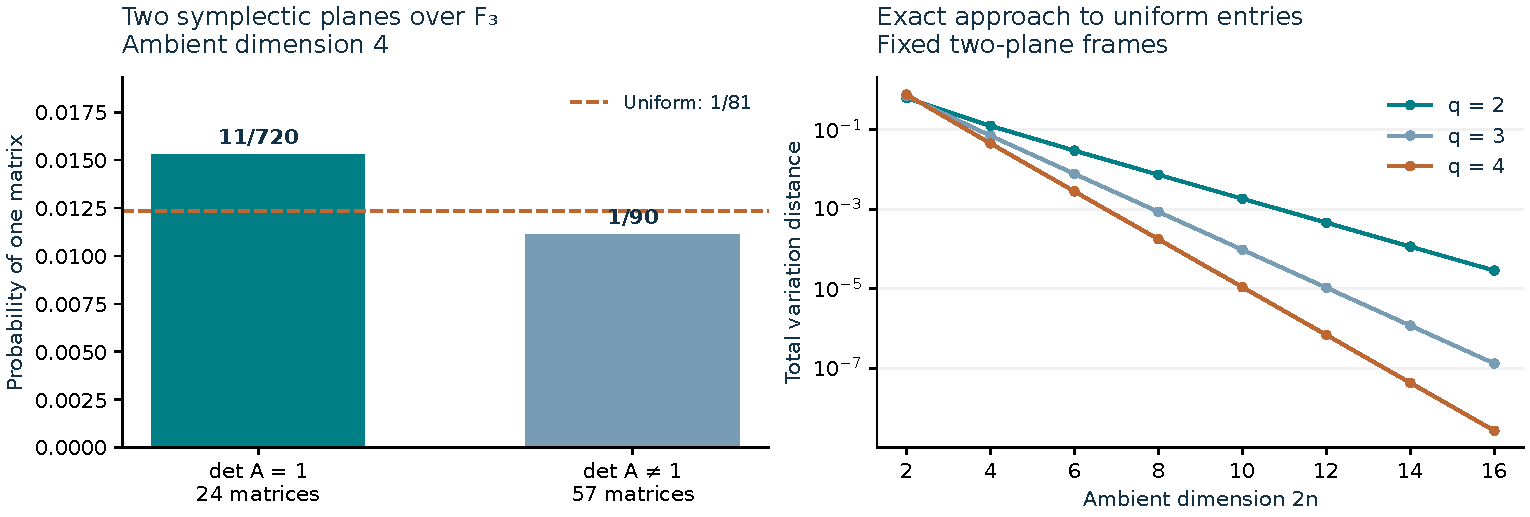
\includegraphics[width=\linewidth]{figures/two_plane_law.pdf}
\caption{Exact two-plane laws. Left: per-matrix probabilities for the example over $\F_3$ in ambient dimension four. Right: the exact total variation distance as the ambient dimension increases; the sharp rate is $q^{-2n}$. Lines connect exact finite formulas and are not Monte Carlo estimates.}
\label{fig:two-plane}
\end{figure}

\section{What the result establishes and what remains}

The exact law applies to every finite field, every feasible pair of frame dimensions, and every pair of restricted alternating forms. It gives probabilities of individual matrices, a complete conditional overlap law, and a necessary and sufficient support test. The minimum-dimension formula has a constructive witness. For fixed field and fixed nonempty frame dimensions, the discrepancy from uniform has a positive, explicitly computable leading coefficient at scale $q^{-2n}$.

This is a transfer of a finite method from the supplied GRH proof, not a consequence that needs RH as an assumption. The proof exposes a reusable distinction: the combined Gram matrix controls the geometric relations, while the intersections of its radical with the two coordinate blocks control whether each original frame remains injective after quotienting.

Three further questions remain separate. First, the constants in fixed-size asymptotics depend on the frame sizes, so those estimates alone do not settle every boundary regime with $a,b$ growing alongside $n$. Second, positive-type \emph{nonuniform} weights in the original source require representation-theoretic information beyond the orbit counts used here. Third, extension to symmetric or Hermitian forms needs the relevant isometry types, and in characteristic two quadratic data cannot be replaced by a symmetric matrix alone.

The contribution is a proved extension relative to the inspected research corpus, supported by a targeted literature comparison. External review could identify an equivalent enumeration in the broader finite-geometry literature; the classical ingredients have therefore been identified explicitly. This note does not assert resolution of any further Riemann hypothesis.

\begin{thebibliography}{9}
\raggedright
\interlinepenalty=10000
\bibitem{grh}
L. Sernau and collaborators, \emph{GRH for Dirichlet $L$-functions, in Lean~4}, based on the proof of L. Alp\"oge with Claude. Repository \texttt{lsernau/grh-lean}, commit \texttt{72fead102f663d5c7a407964a13dc0cf9d977207}, 25 November 2026. \url{https://github.com/lsernau/grh-lean}. In particular, \texttt{grh/GUIDE.md}, \texttt{grh/src/Statements.lean}, and \texttt{grh/src/New/Spanning/SecondMoment/PositiveType.lean}.

\bibitem{proveit}
V. Reshetnikov, \emph{ProveIt: Generalized Riemann Hypothesis research collection}, commit \texttt{041d8032541746f2ac2e686fbe437f8092771670}, inspected 26 November 2026 (Pacific time). \url{https://github.com/VladimirReshetnikov/ProveIt/tree/main/Analysis/GeneralizedRiemannHypothesis}. The merged article's Section \texttt{spn.tex}, especially Question \texttt{spn:q:symplectic}, and its listed predecessor packets.

\bibitem{rankblind}
\emph{Symplectic rank blindness}, research packet delivered 26 November 2026, in ProveIt, \texttt{Analysis/GeneralizedRiemannHypothesis/docs/incoming/}\allowbreak\texttt{symplectic\_rank\_blindness\_2026-11-26.zip}. Git blob \texttt{ec19f1ebda1c32ab29b3bc00575962b411c73b7c}. Its \texttt{paper.tex} gives the exact Lagrangian-output law and explicitly leaves both compressed spaces arbitrary.

\bibitem{glt}
R. M. Guralnick, M. Larsen, and P. H. Tiep, \emph{Character levels and character bounds for finite classical groups}, Inventiones Mathematicae \textbf{235} (2024), 151--210, especially Lemma~2.6. \url{https://doi.org/10.1007/s00222-023-01221-5}.

\bibitem{deboeck}
M. De Boeck and G. Van de Voorde, \emph{Anzahl theorems for trivially intersecting subspaces generating a non-singular subspace I: Symplectic and hermitian forms}, Linear Algebra and its Applications \textbf{699} (2024), 367--402. \url{https://doi.org/10.1016/j.laa.2024.07.004}. Author version: \url{https://arxiv.org/abs/2407.07486}.

\bibitem{ishizuka}
K. Ishizuka, \emph{Uniform Sampling of Linear Codes with Prescribed Hull Dimension}, arXiv:2611.03578v2, 25 November 2026. \url{https://arxiv.org/abs/2611.03578}.

\bibitem{zhang}
Y. Zhang, S. Liu, and L. Zeng, \emph{A symplectic fission scheme for the association scheme of rectangular matrices and its automorphisms}, AIMS Mathematics \textbf{9}(11) (2024), 32819--32830. \url{https://doi.org/10.3934/math.20241570}.

\bibitem{wiki}
Wikipedia contributors, \emph{Riemann hypothesis}, page inspected 26 November 2026. \url{https://en.wikipedia.org/wiki/Riemann_hypothesis}. Used for the user-supplied contextual overview, not as a proof source for the new theorem.
\end{thebibliography}

\end{document}
